% Created 2022-11-16 mer 14:31
% Intended LaTeX compiler: pdflatex
\documentclass[presentation]{beamer}
\usepackage[utf8]{inputenc}
\usepackage[T1]{fontenc}
\usepackage{graphicx}
\usepackage{longtable}
\usepackage{wrapfig}
\usepackage{rotating}
\usepackage[normalem]{ulem}
\usepackage{amsmath}
\usepackage{amssymb}
\usepackage{capt-of}
\usepackage{hyperref}
\usepackage{minted}
\usepackage[, french]{babel}
\usepackage{svg}
\logo{
\includegraphics[width=.1\textwidth]{../../by-sa.png}}
\usetheme{metropolis}
\usecolortheme{}
\usefonttheme{}
\useinnertheme{}
\useoutertheme{}
\author{Guy Bégin}
\date{\today}
\title{Circuits logiques combinatoires et séquentiels}

\hypersetup{
 pdfauthor={Guy Bégin},
 pdftitle={Circuits logiques combinatoires et séquentiels},
 pdfkeywords={},
 pdfsubject={},
 pdfcreator={Emacs 28.1 (Org mode 9.5.4)}, 
 pdflang={French}}
\begin{document}

\maketitle

\section{Mémoires}
\label{sec:org4eadd9a}
\begin{frame}[label={sec:orgbf66310}]{Objectifs}
\begin{itemize}
\item Pouvoir distinguer entre mémoire volatile et non-volatile
\item Pouvoir distinguer entre mémoire volatile statique et dynamique
\item Connaître l'organisation typique d'une mémoire et le fonctionnement
de l'adressage
\item Comprendre le fonctionnement d'un bus de données
\item Pouvoir interpréter les cycles d'écriture et de lecture
\item Pouvoir implémenter une fonction combinatoire arbitraire à l'aide d'une
mémoire ROM
\item Pouvoir utiliser un tableau de correspondance
\item Être familier avec les différents types de mémoires non-volatiles
\end{itemize}
\end{frame}

\begin{frame}[label={sec:orga0b55d3}]{Mémoires}
\begin{itemize}
\item Une mémoire est utilisée pour stocker des valeurs binaires à plus ou moins long terme.

\item Généralement, l'information stockée dans la mémoire sera lue et acheminée dans des registres pour être traitée par un circuit logique de traitement.

\item Les résultats du traitement seront typiquement stockés de nouveau dans la mémoire.

\item Constituée d'un grand nombre de cellules permettant chacune de stocker un bit, la mémoire est dotée de mécanismes permettant d'accéder aux cellules pour en faire la lecture ou l'écriture.

\item On distingue les mémoires non-volatiles (en anglais, \emph{Read Only Memories}, (ROM)) et les mémoires volatiles (en anglais, \emph{Random Access Memories}, (RAM)).
\end{itemize}
\end{frame}

\begin{frame}[label={sec:org5efd6d3}]{Mémoires non-volatiles}
\begin{itemize}
\item Dans une mémoire ROM, les données sont stockées une fois pour toute.

\item Elles y demeurent même après que la mémoire ait été mise hors tension.

\item Dans le cycle de vie des données, il y a donc \alert{une} écriture initiale, mais autant de lectures qu'on le souhaite.

\item Il ne peut pas y avoir de récriture.
\end{itemize}
\end{frame}

\begin{frame}[label={sec:orgbfe93e7}]{Mémoire ROM}
\begin{itemize}
\item Une mémoire ROM est considérée comme un dispositif \alert{programmable}, dans le sens que le processus d'écriture initial demande une action particulière, une procédure spécifique au niveau matériel.

\item On verra plus loin d'autres dispositifs logiques programmables.

\item La programmation d'une ROM se fait en agissant sur des connexions dites \alert{fusibles}.

\item Initialement, le fusible est comme un fil qui permet au signal de passer.

\item En le programmant, le fusible devient un circuit ouvert qui ne laisse plus passer le signal.
\end{itemize}
\end{frame}

\begin{frame}[label={sec:orge061c44}]{Mémoires volatiles}
\begin{itemize}
\item Une mémoire RAM stocke l'information de façon temporaire.

\item En principe, le contenu est conservé tant que la mémoire est maintenue sous tension. Mais la réalité est un peu plus complexe, comme on le verra plus loin.

\item L'opération d'\alert{écriture} permet de stocker des valeurs, et la \alert{lecture} permet d'extraire l'information de la mémoire.
\end{itemize}
\end{frame}

\begin{frame}[label={sec:org3f14c14}]{RAM statique}
\begin{itemize}
\item Une mémoire RAM \alert{statique} consiste en un ensemble de loquets qui permettent de conserver des données binaires.

\item L'information est maintenue tant que la mémoire est alimentée.
\end{itemize}
\end{frame}

\begin{frame}[label={sec:orgc4d8567}]{RAM dynamique}
\begin{itemize}
\item Les mémoires RAM \alert{dynamiques} stockent l'information sous la forme d'une charge capacitive au sein des transistors du circuit intégré.

\item Comme cette charge se disperse au fil du temps, la mémoire doit être rafraîchie régulièrement, en y récrivant périodiquement à très court intervalle (millisecondes) la même valeur qui est déjà stockée.

\item Les mémoires dynamiques consomment beaucoup moins que les mémoires statiques et offrent des capacités de stockage largement supérieures, car une cellule de mémoire comporte beaucoup moins d'éléments (essentiellement un transistor par cellule).

\item En contrepartie, les temps d'accès aux mémoires statiques sont nettement meilleurs et on n'a pas à se préoccuper de rafraîchissement.
\end{itemize}
\end{frame}

\begin{frame}[label={sec:org25161f3}]{Adressage}
\begin{itemize}
\item Les cellules des mémoires sont organisées en petits groupes appelés \alert{mots}, de façon à ce que l'on puisse accéder à chaque groupe indépendamment.

\item Toutes les cellules d'un mot sont lues ou écrites ensemble.

\item Cet accès individuel aux mots, appelé \alert{adressage}, est une caractéristique de flexibilité essentielle.

\item Le temps d'accès aux données est le même, quel que soit l'endroit dans la mémoire où un mot en particulier est stocké.

\item Les mots sont généralement constitués d'un nombre de bits multiple de huit: 8, 16 ou 32 bits sont des tailles de mots courantes.

\item Un groupe de huit bits est appelé \alert{octet}.
\end{itemize}
\end{frame}

\begin{frame}[label={sec:orgab3ce34}]{Décodeur d'adresses}
\begin{itemize}
\item L'adressage se fait au moyen d'un \alert{décodeur d'adresses}, qui est simplement un décodeur binaire tel que vu précédemment.

\item Le nombre de bits d'adresse détermine la capacité (en nombre de mots) de la mémoire: pour \(k\) adresses, on aura \(2^k\) mots distincts.

\item Les tailles de mémoire sont souvent exprimées au moyen de multiplicateurs: K (kilo) correspondant à \(2^{10}\), M (mega) correspondant à \(2^{20}\) ou G (giga) correspondant à \(2^{30}\).
\end{itemize}
\end{frame}


\begin{frame}[label={sec:orgcf752f1}]{Schéma d'une mémoire}
\begin{figure}[htbp]
\centering
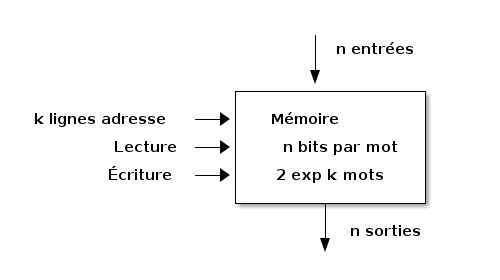
\includegraphics[scale=0.65]{../../Sources_images_logiques/images/memoire.png}
\caption{\label{fig:org5cec4d4}Schéma d'une mémoire}
\end{figure}
\end{frame}

\begin{frame}[label={sec:orgf54d2b2}]{Lecture et écriture}
\begin{itemize}
\item L'opération choisie, écriture ou lecture, est commandée par une ou des entrées à cet effet.

\item L'accès à un espace-mémoire (un mot) se fait selon une séquence bien précise.
\end{itemize}
\end{frame}

\begin{frame}[label={sec:orgef1239b},fragile]{Écriture}
 Pour une écriture:

\begin{enumerate}
\item Les bits d'adresse du mot sont appliqués aux lignes d'adresses.
\item Les données à écrire sont appliquées aux lignes d'entrée.
\item On active l'entrée de commande \texttt{Écriture}.

\item Les données de l'entrée sont alors stockées dans la case-mémoire adressée.
\end{enumerate}
\end{frame}

\begin{frame}[label={sec:org849783e},fragile]{Lecture}
 Pour une lecture:

\begin{enumerate}
\item Les bits d'adresse du mot sont appliqués aux lignes d'adresses.
\item On active l'entrée de commande \texttt{Lecture}.
\end{enumerate}

Les données présentes dans la case-mémoire adressée sont ensuite
disponibles à la sortie de la mémoire.
\end{frame}

\begin{frame}[label={sec:orgce8c927},fragile]{Signal de contrôle combiné}
 \begin{itemize}
\item Les mémoires disponibles sur le marché optent souvent pour une combinaison des signaux de contrôle, avec un seul signal qui détermine le sens de l'action, comme on peut le voir dans le tableau \ref{tab:org4372254}.

\item Le signal \texttt{Enable}, parfois appelé \texttt{Chip select}, permet d'activer une mémoire dans un ensemble où plusieurs mémoires sont utilisées.
\end{itemize}
\end{frame}

\begin{frame}[label={sec:org6176e00},fragile]{Signaux de contrôle d'une mémoire}
 \begin{table}[htbp]
\caption{\label{tab:org4372254}Signaux de contrôle d'une mémoire}
\centering
\begin{tabular}{rrl}
\texttt{Enable} & \texttt{Lecture/écriture} & Action\\
\hline
0 & X & Aucune\\
1 & 0 & Écriture\\
1 & 1 & Lecture\\
\end{tabular}
\end{table}
\end{frame}

\begin{frame}[label={sec:org67d5ff1},fragile]{Bus de données}
 \begin{itemize}
\item Pour acheminer les données lues ou à écrire dans la mémoire, on utilise des tampons émetteur-récepteurs de bus, organisés en vecteur, pour créer un \alert{bus de données} qui permet un aller-retour des données, selon le sens de l'action.

\item Cela permet de diminuer de moitié le nombre de connexions nécessaires pour l'échange des données.

\item Un signal dérivé des signaux \texttt{Lecture/écriture} et \texttt{Chip select (CS)} est typiquement utilisé pour commander l'entrée de contrôle (voir figure \ref{fig:org232c257}).
\end{itemize}
\end{frame}

\begin{frame}[label={sec:orgeaf2029}]{Bus de données, 8 bits}
\begin{figure}[htbp]
\centering
\includesvg[scale=0.75]{../../Sources_images_logiques/images/bus_trans8}
\caption{\label{fig:org232c257}Bus de données, 8 bits}
\end{figure}
\end{frame}

\begin{frame}[label={sec:orgd8faa9b},fragile]{Chronogrammes}
 \begin{itemize}
\item La figure \ref{fig:orgd051d75} présente un chronogramme qui décrit l'opération d'écriture dans une mémoire RAM.

\item Les valeurs d'adresses sont d'abord présentée aux entrées d'adressage.

\item Le signal \texttt{L/not E} est amené au niveau bas, en même temps que le signal \texttt{CS} est activé (au niveau bas).

\item Après un court délai, les données sont mises sur le bus de données et seront écrites dans la mémoire.

\item On peut voir que les lignes du bus de données sont en mode \alert{haute impédance} lorsque le bus est inactif (situation représentée symboliquement sur l'illustration par un signal situé entre les niveaux 0 et 1).
\end{itemize}
\end{frame}

\begin{frame}[label={sec:org5cce603}]{Mémoire RAM, chronogramme pour l'écriture}
\begin{figure}[htbp]
\centering
\includesvg[scale=0.75]{../../Sources_images_logiques/images/chron_ram_ecriture}
\caption{\label{fig:orgd051d75}Mémoire RAM, chronogramme pour l'écriture}
\end{figure}
\end{frame}

\begin{frame}[label={sec:orgf6a0748},fragile]{Mémoire RAM, chronogramme pour la lecture}
 \begin{itemize}
\item La figure \ref{fig:org0a2be70} présente un chronogramme qui décrit l'opération de lecture d'une mémoire RAM.

\item Les valeurs d'adresses sont d'abord présentée aux entrées d'adressage.

\item Le signal \texttt{L/not E} est maintenu au niveau élevé en même temps que le signal \texttt{CS} est activé (au niveau bas).

\item Après un court délai, les données sont disponibles sur le bus de données.
\end{itemize}
\end{frame}

\begin{frame}[label={sec:orgd3a757e}]{Mémoire RAM, chronogramme pour la lecture}
\begin{figure}[htbp]
\centering
\includesvg[scale=0.75]{../../Sources_images_logiques/images/chron_ram_lecture}
\caption{\label{fig:org0a2be70}Mémoire RAM, chronogramme pour la lecture}
\end{figure}
\end{frame}

\begin{frame}[label={sec:orgc39f6c4}]{Cellule de base}
\begin{itemize}
\item La cellule de base d'une mémoire RAM qui permet de stocker un bit est illustrée à la figure \ref{fig:orgf3540f4}.

\item Elle est construite autour d'un loquet SR et de portes logiques pour le contrôle.

\item Une mémoire complète de \(m\) mots de taille \(n\) bits sera constituée d'une matrice de format \(m \times n\) de telles cellules, avec un décodeur d'adresses pour sélectionner quel mot sera affecté par l'opération choisie.
\end{itemize}
\end{frame}

\begin{frame}[label={sec:org28e8cc4}]{Cellule mémoire RAM}
\begin{figure}[htbp]
\centering
\includesvg[scale=0.75]{../../Sources_images_logiques/images/cell_ram}
\caption{\label{fig:orgf3540f4}Cellule mémoire RAM}
\end{figure}
\end{frame}


\begin{frame}[label={sec:org8962976},fragile]{Mémoires mortes}
 \begin{itemize}
\item Dans son mode d'utilisation normal, une mémoire morte peut seulement être lue.

\item Il n'est donc pas nécessaire de préciser l'opération qui sera effectuée.

\item Il y aura donc des entrées pour les adresses et un signal de contrôle de type \texttt{CS}.

\item La figure \ref{fig:orgf30d6b0} montre l'essentiel d'une mémoire ROM de 16 mots de 4 bits.

\item Cette relativement petite mémoire comporte ainsi 64 intersections programmables, permettant de définir la valeur des 16 mots de mémoire de 8 bits chacun.
\end{itemize}
\end{frame}

\begin{frame}[label={sec:org74664a6}]{Modèle d'une mémoire ROM}
\begin{figure}[htbp]
\centering
\includesvg[scale=0.75]{../../Sources_images_logiques/images/proto_rom1_prog}
\caption{\label{fig:orgf30d6b0}Modèle d'une mémoire ROM}
\end{figure}
\end{frame}


\begin{frame}[label={sec:org15dbc96}]{Mémoires mortes \ldots{} 2}
\begin{itemize}
\item Un décodeur d'adresse permet de sélectionner quel mot sera lu, et la sortie est disponible sur les lignes \(A_3, \ldots, A_0\).

\item Pour simplifier la représentation de ce genre de configuration, on utilise une schématisation symbolique compacte pour les portes OU de sortie, dans laquelle chacune des 16 lignes horizontales représente en fait 16 entrées d'une porte OU.

\item La présence d'une croix à l'intersection d'une ligne horizontale et d'une ligne verticale signifie que le signal de la ligne horizontale est connecté à une des entrées de la porte.

\item Avec cette schématisation, on peut voir que les deux premiers mots stockés dans la mémoire illustrée dans l'exemple seraient 0101 et 1101.

\item La même schématisation compacte s'emploie aussi pour des portes ET.
\end{itemize}
\end{frame}

\begin{frame}[label={sec:org8081606}]{Implémentation de fonctions combinatoires}
\begin{itemize}
\item Comme on l'a vu précédemment, un décodeur permet de générer les \(2^k\) minterms possibles avec ses \(k\) entrées.

\item Regrouper avec une porte OU les minterms d'une fonction permet d'implémenter cette fonction.

\item Une mémoire ROM permet de faire exactement cela sans avoir rien à ajouter, car elle est munie d'un décodeur d'entrées et la porte OU de sortie fait déjà partie de la ROM.
\end{itemize}
\end{frame}

\begin{frame}[label={sec:org19e57ee}]{Implémentation de fonctions combinatoires \ldots{} 2}
\begin{itemize}
\item On peut donc interpréter le fonctionnement d'une mémoire ROM de \(k\) bits d'adresse et avec des mots de taille \(m\) comme un dispositif qui permet, pour les entrées qui sont ses adresses, de mettre en oeuvre \(m\) fonctions combinatoires différentes (une par bit de mot) de \(k\) entrées.

\item Par exemple, la sortie \(A_2\) de la mémoire de la figure \ref{fig:orgf30d6b0} implémente la fonction $$ A_2 = \sum (0,1,4,8) $$ exprimée en somme de minterms.
\end{itemize}
\end{frame}

\begin{frame}[label={sec:org64d5c7b}]{Tableau de correspondance}
\begin{itemize}
\item Cette approche qui consiste à réaliser une fonction logique combinatoire au moyen d'une mémoire qui spécifie, pour chaque combinaison d'entrée possible, une valeur de sortie, est largement utilisée dans les composants programmables.

\item On parle alors de tableau de correspondance (en anglais, \emph{LookUp Table}, (LUT)).

\item Il s'agit ni plus ni moins que de stocker en mémoire le tableau de vérité de la fonction à réaliser.

\item Dans les composants programmables, on utilise plutôt des mémoires RAM pour les tableaux de correspondance, afin que la configuration des fonctions puisse être changée selon l'application.
\end{itemize}
\end{frame}

\begin{frame}[label={sec:orgbd12acf}]{Catégories de mémoires ROM}
\begin{itemize}
\item On distingue quatre grandes approches technologiques pour réaliser des mémoires mortes.

\item Leurs usages typiques sont surtout déterminés par la façon de les configurer (on dit couramment \emph{programmer}, même s'il s'agit d'un intervention au niveau du matériel).
\end{itemize}
\end{frame}

\begin{frame}[label={sec:org1bb626f}]{Programmation par masque}
\begin{itemize}
\item Dans la \alert{programmation par masque}, la mémoire est programmée lors de la fabrication de la puce.

\item Le fabricant se base sur un tableau de vérité fourni par le client pour établir des connexions qui seront implémentées (ou pas) dans le procédé de fabrication via des masques qui empêchent la déposition de matériau conducteur sur les couches du circuit intégré.

\item Cette approche convient à la production de masse à grand volume.
\end{itemize}
\end{frame}

\begin{frame}[label={sec:org29982ae}]{Programmation sur mesure}
\begin{itemize}
\item Dans la \alert{programmation sur mesure}, on utilise un type de mémoire qui comporte initialement des connexions entre toutes les sorties du décodeur et toutes les entrées des portes OU de sortie (la mémoire en configuration initiale comporte des 1 partout).

\item La programmation, qui peut se faire chez le développeur au moyen d'un dispositif de programmation (ou programmeur) spécialement conçu à cette fin, consiste à supprimer les connexions qui ne sont pas nécessaires en envoyant des impulsions à forte tension pour faire fondre les fusibles de connexions spécifiques.

\item Un fusible fondu (pas de connexion) correspondant à un bit 0 dans la mémoire.

\item Cette programmation est bien entendu irréversible: impossible de reconnecter une fois que le fusible est fondu.
\end{itemize}
\end{frame}

\begin{frame}[label={sec:orgb48e8eb}]{PROM}
\begin{itemize}
\item Avec un \alert{PROM} (pour \emph{Programmable ROM}), il est possible d'effacer la configuration dans son ensemble en soumettant la puce à une lumière ultraviolet pendant un certain temps.

\item Ce bombardement énergétique permet de décharger les grilles flottantes des dispositifs qui implémente les connexions.

\item La mémoire PROM peut être reconfigurée de nouveau.

\item Avec la \alert{programmation électrique}, il est possible de reconfigurer l'ensemble d'une mémoire dite EEPROM (\emph{Electrically Erasable PROM}) en la soumettant à un signal électrique d'effacement.
\end{itemize}
\end{frame}

\begin{frame}[label={sec:orgdcf80ba}]{Programmation \emph{flash}}
\begin{itemize}
\item Les ROM à \alert{programmation \emph{flash}} sont semblables aux EEPROM, mais la reconfiguration peut se faire adresse par adresse.

\item Il est notamment possible de reconfigurer une mémoire sans la retirer de son circuit.  Fonctionnellement, ces mémoires sont à mi-chemin entre la mémoire RAM et la mémoire sur disque.

\item Les mémoires \emph{flash} tendent d'ailleurs de plus en plus à remplacer ce dernier type dans les systèmes portables: téléphones, ordinateurs portables, etc.
\end{itemize}
\end{frame}
\end{document}